\documentclass[11pt,journal]{IEEEtran}
\usepackage{lipsum}
\usepackage[T1]{fontenc}
\usepackage{fouriernc}
\usepackage{cases}
\usepackage{amsmath}
\usepackage[noadjust]{cite}
\usepackage{hyperref}
\usepackage{multirow}
\usepackage{graphicx}
\usepackage{adjustbox}
\usepackage{makecell}
\usepackage[dvipsnames]{xcolor}
\usepackage{tikz}
\usepackage{lipsum}
\usepackage{listings}

\hypersetup{
    colorlinks=true,
    linkcolor=blue,
    anchorcolor=blue,
    urlcolor=blue,
    citecolor=blue
}

\newcommand{\eq}{\; = \;}
%\newcommand{\text}[1]{\mbox{\footnotesize #1}}
\newcommand{\nl}{

\medskip

}
\newcommand{\centered}[2]{\begin{tabular}{#1} #2 \end{tabular}}

\lstdefinestyle{standstyle}{
    %backgroundcolor=\color{backcolour!05},
    basicstyle=\ttfamily\linespread{1}\scriptsize\color{black!80},
    breakatwhitespace=false,
    breaklines=true,
    captionpos=b,
    keepspaces=true,
    numbers=none,
    numbersep=5pt,
    showspaces=false,
    showstringspaces=false,
    showtabs=false,
    tabsize=4,
}

\lstset{style=standstyle}

\DeclareMathAlphabet{\mathcal}{OMS}{zplm}{m}{n}

\title{GuNiLeo: An Attempt To Perform Lip Reading From Videos With STCNN}
\author{Beray Nil Atabey (\textit{2045576}) \quad Leonardo Biason (\textit{2045751}) \quad Günak Yüzak (\textit{2048950})}

\begin{document}

\maketitle

\begin{abstract}
    Lip reading is a task that can have various usages as an accessibility feature, but it's also very complex to design: it requires a machine to be able to differentiate between the various words said by a speaker, and also to predict what the speaker said whenever words aren't spelled with a precise motion of the lips. With this paper, we propose a model based on a Spatio-Temporal CNN, capable of reading the words said by a speaker from a video clip of maximum 75 frames.
\end{abstract}

\begin{keywords}
    Sapienza, AcsAi, STCNN, Lip reading, CTC Loss, Computer Vision 
\end{keywords}

\section{Introduction}

With this paper, we describe an attempt on building a lip reading architecture, using videos up to 75 frames, using a dataset of 5000+ videos. For the model the PyTorch framework was used, along with a helper pre-trained model for landmarking the face. The model uses convolutional and recurrent neural networks, where convolution is in 3D and recurrency is bidirectional.
Our model takes inspiration from the LipNet paper \cite{lipnet}, which also employs many of the techniques that we used. The LipNet acquired a $95\%$ accuracy metric, which is by no doubt an accomplishment. In this paper, however, we don't have an accuracy metric, as it will be explained further.

 
\section{Implementation }

In order to create a lip reading model, the following steps have been undertaken:
\begin{itemize}
    \item [1)] creation and modeling of the dataset;
    \item [2)] creation of the model;
    \item [3)] training of the model;
    \item [4)] evaluation of the model.
\end{itemize}

\section{Creation and Modeling of the Dataset}

The project adopted an already existing dataset from the University of Sheffield: such dataset is called \textsc{Lombard Grid} \cite{gunileo:dataset}.

\subsection{Structure of the Dataset}

The dataset comprehends two fundamental parts: the data part and the labels. The data consists in a set of 5000+ videos, where each video records frontally a person saying a specific sentence. This sentence is made up of 6 parts, which are in order: \textsc{command}, \textsc{color}, \textsc{preposition}, \textsc{letter}, \textsc{digit}, \textsc{adverb}. The possible values are the following:
\begin{itemize}
    \item \textbf{Command}: \texttt{bin}, \texttt{lay}, \texttt{place}, \texttt{set};
    \item \textbf{Color}: \texttt{blue}, \texttt{green}, \texttt{white}, \texttt{red};
    \item \textbf{Preposition}: \texttt{at}, \texttt{by}, \texttt{in}, \texttt{with};
    \item \textbf{Letter}: \texttt{a}-\texttt{z} except \texttt{w};
    \item \textbf{Digit}: \texttt{0}-\texttt{9};
    \item \textbf{Adverb}: \texttt{again}, \texttt{now}, \texttt{please}, \texttt{soon}.
\end{itemize}

\nl
There are 4 words for command, color and preposition, 25 values for letter, 10 values for digit and 4 words for adverb, thus having 64000 different combinations. Each video comes with its pair, alignment data which after this we will refer as labels. Each label is transcribed in a \texttt{json} file, which has the following format:

\begin{itemize}
    \item \texttt{video\_name}: a list containing all the phonemes and the timing of said phonemes of a clip;
    \begin{itemize}
        \item \texttt{duration}: the duration in seconds of the phoneme;
        \item \texttt{offset}: the beginning of the phoneme, with respect to the beginning of the video;
        \item \texttt{phone}: an encoding of the phoneme.
    \end{itemize}
\end{itemize}

\begin{figure}
    \renewcommand{\arraystretch}{1.3}
    \caption{Example of frame (on the left) and label (on the right)}
    \label{frame_label}

    \begin{tabular}{c c}
        \centered{c}{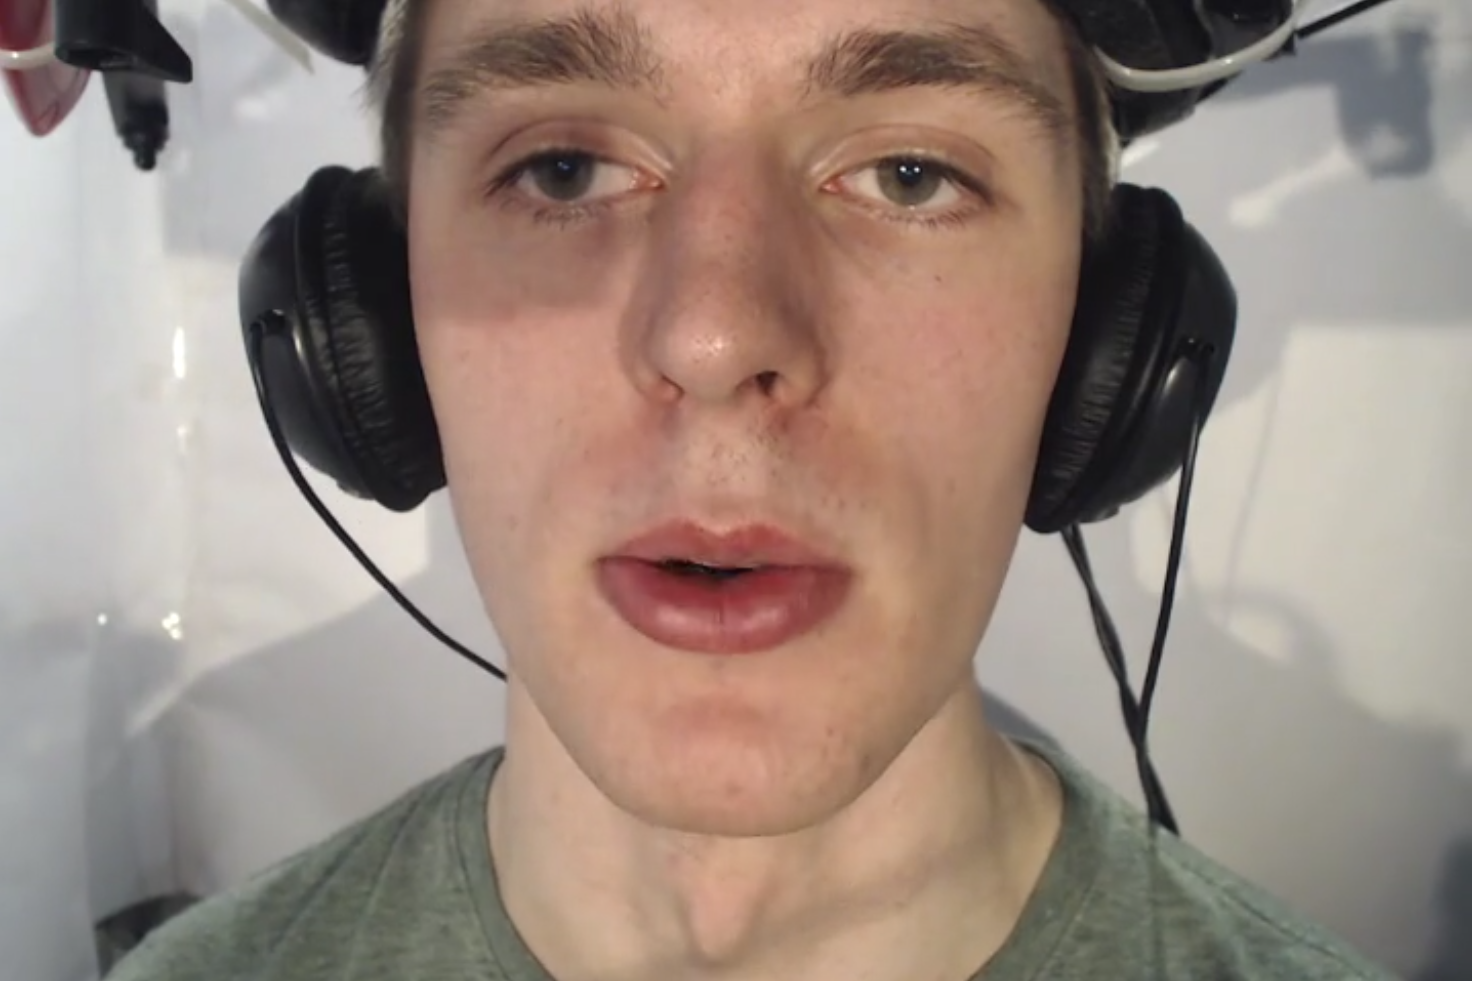
\includegraphics[width = 0.3\linewidth]{images/001_frame.PNG}} & \begin{lstlisting}[language = python]
{
    "video_name": [
        {
            "duration": 0.01,
            "offset": 0,
            "phone": "SIL_S"
        }
    ]
}
            \end{lstlisting} \\
        {\scriptsize Frame} & {\scriptsize Label} \\
    \end{tabular}
\end{figure}

\nl
An example of data-label pair can be observed in Figure \ref{frame_label}, where a frame of a sample video has been reported, alongside an example of possible label. The label can be interpreted as follows: there is a phoneme, the silent "s", which starts at $t \eq 0$ and lasts for $0,01s$.

\begin{figure}
    \centering{
        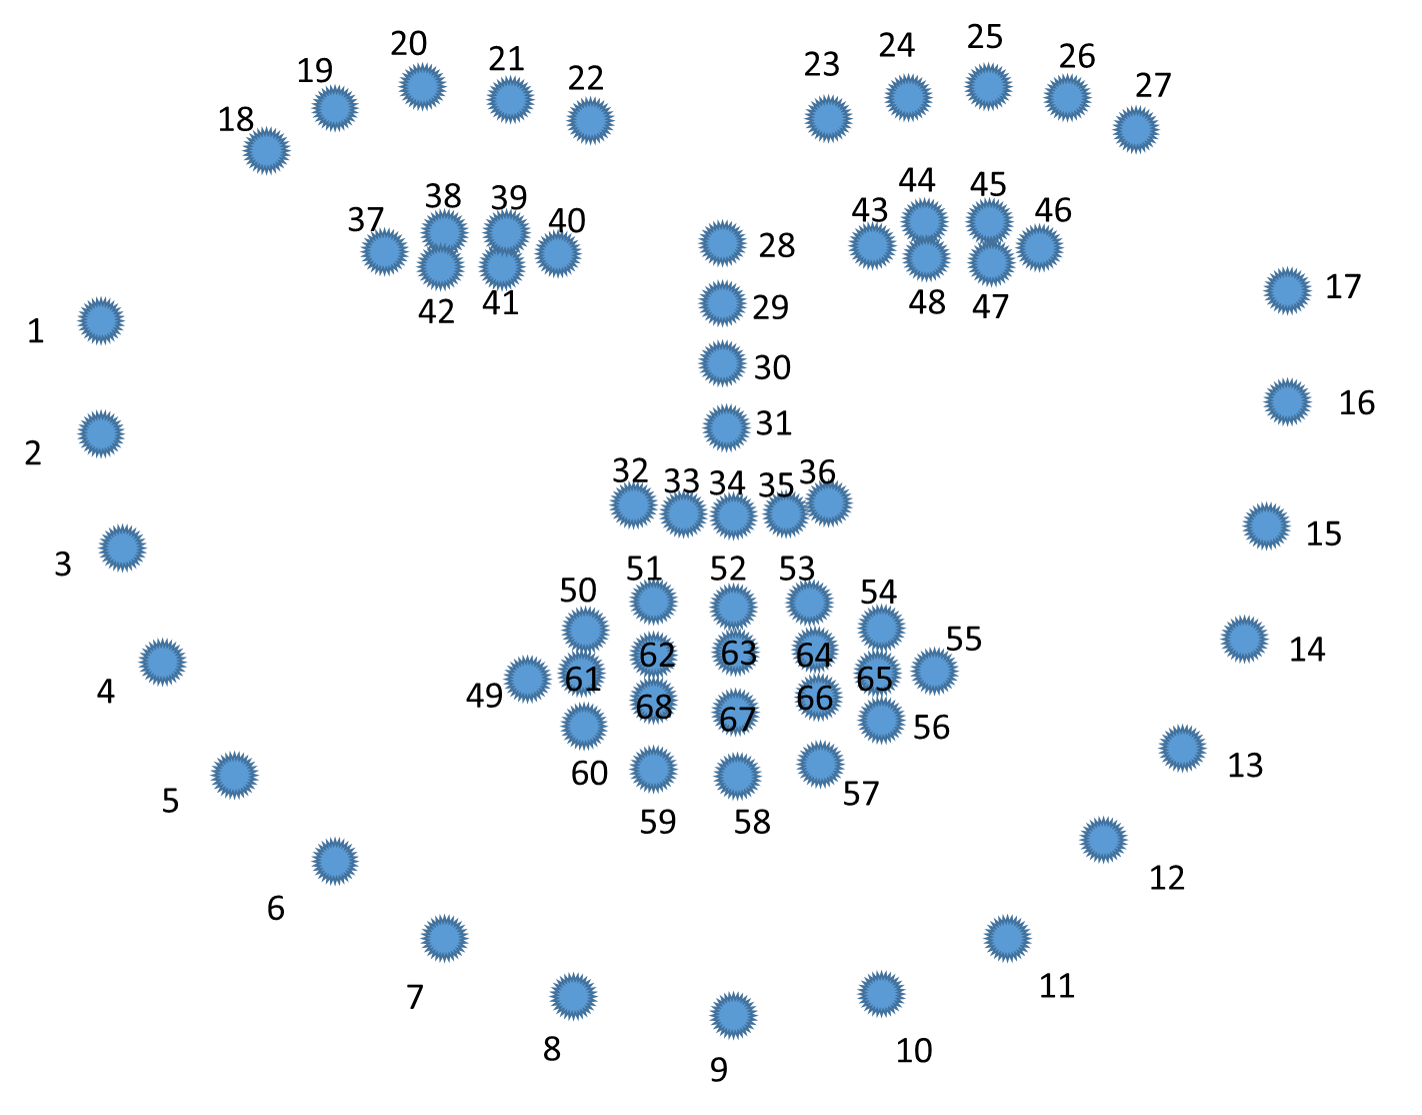
\includegraphics[width = 0.7\linewidth]{images/002_face_landmark_representation.png}
    }
    \renewcommand{\arraystretch}{1.3}
    \caption{Face landmarking points}
    \label{face_landmark_points}
\end{figure}

\begin{figure*}
    \centering{
        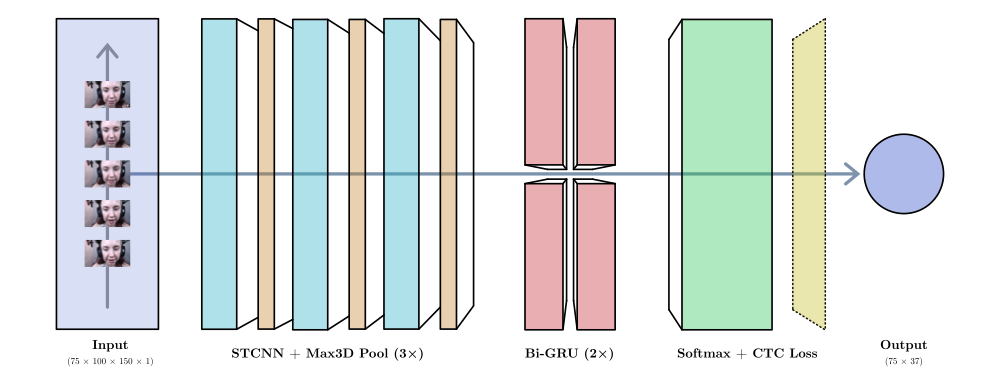
\includegraphics[width = \linewidth]{images/003_model.png}
    }
    \renewcommand{\arraystretch}{1.3}
    \caption{Visual representation of the model}
    \label{model_struct}
\end{figure*}

\subsection{Pre-processing of the Dataset}

The pre-processing of the dataset took place in two steps: first, the pre-processing of the data, then, the pre-processing of the labels.

\nl
\textbf{Pre-processing of the Videos}: Since we want to read the lips, the only area that concerns us is the mouth and the close surroundings. The rest of the video can be cropped to avoid unnecessary memory-wise and computational power-wise waste. In order to locate the mouth, the \texttt{dlib} \cite{gunileo:dlib} library's face detection and landmark detection algorithm has been employed. The face detection is implemented in \texttt{dlib} itself, however for the landmark an external model had to be used. We now proceed to describe the undertaken steps for the pre-processing of the data:
\begin{itemize}
    \item [1)] First, the face detection algorithm is ran on the video in order to find the coordinates of the face;
    \item [2)] Such coordinates are given as input into the landmark model, which determines the important landmarks of the face via a sequence of 68 points. Points from 49 to 68 determine where the mouth is (such points are shown in Figure \ref{face_landmark_points});
    \item [3)] From these points, it's possible to find the points that are on the left,right, up and down most of the mouth, which correspond to the maximum coordinates that a mouth can take in a specific video;
    \item [4)] From these coordinates a margin distance is added, and after that the video gets cropped around the mouth. Clearly, every person's mouth size is different from one another, so the resize procedure reshapes the video to a fixed size of $150 \times 100$ pixels;
    \item [5)] Finally, the resized video is then gray scaled and normalized for a better performance of the model.
\end{itemize}

\textbf{Pre-processing of the Labels}: Rather than dealing with the phonetics as presented in the \texttt{json}'s, we tried a different approach. We extracted what was being said in the videos from their file name, since the file name is made up by taking the first letter from the 6 spoken words. Every word in the categories are different in the same category by the first letter so no confusion is made this way. We then craft our label as a list of the characters in the said sentence, including the spaces.

\section{Architecture of the Model}

The model used for this project takes large advantage of the \textsc{Spatio-Temporal Convolutional Neural Network} concept \cite{gunileo:stcnn} (from now on referred to as STCNN). The choice of using such type of neural network is because of its capabilities of retaining information in the long short-term, which is very helpful when it comes to analysing multiple videos and making predictions on the long run.
\nl
Here follows the detailed architecture of our model, with all its layers:
\begin{itemize}
    \item STCNN and 3D Max Pooling $\times 3$: a STCNN layer has the following equation
\end{itemize}
    \begin{equation}
        [\text{stconv}(\mathbf{x},\mathbf{w})]_{c'tij} = \sum_{c = 1}^C \sum_{t' = 1}^{k_t} \sum_{i' = 1}^{kw} \sum_{j' = 1}^{kh} w_{c'ct'i'j'} \: x_{c,t+t',i+i',j+j'}
    \end{equation}
\begin{itemize}
    \item Bi-directional GRU unit $\times 2$;
    \item CTC loss function;
    \item $\log$-Softmax activation function.
\end{itemize}

\nl
As input, the model takes a clip of size $(100, \; 150, \; 75, \; 1)$, and it returns a tensor of shape $(75, \; 37)$. The possible output, once encoded, is a list composed by letters from a-z, numbers from 0-9 or blank spaces "\textvisiblespace". A summary of the model is shown in Table \ref{model_specs}.
\nl
The model supports 75 frames videos, which is a video of 3 seconds with a constant frame rate of 25$f$. The videos that had more than 75 frames are discarded from the dataset, and less then 75 frames are extended with 0 matrices.

\subsection{Hyperparameters}

The model was trained with the $k$-fold cross validation technique, where $k = 5$, and with the following hyperparameters:
\begin{itemize}
    \item 10 \textbf{epochs};
    \item a \textbf{learning rate} of $10^{-4}$;
    \item a \textbf{dropout} of $0.5$.
\end{itemize}

\nl We opted for the \textbf{AdamW} optimizer, because of its computational efficiency. Given that the training of the model would've required various resources and time, it seemed a reasonable option.

\nl The loss function $\mathcal{L}$ used in the model is a \textbf{Connectionist Temporal Classification} (\textbf{CTC}) Loss function, which employs $\log$ probabilities in order to detect a sequence of characters within a piece of audio or video (in our case, it will be on videos).

\begin{table*}
    \renewcommand{\arraystretch}{1.3}
    \caption{Values and Dimensions of the Model}
    \label{model_specs}
    \centering
    \begin{tabular}{|c|c c c c c|}
        \hline
        \textbf{Layer} & \textbf{Size} & \textbf{Stride} & \textbf{Padding} & \textbf{Input} & \textbf{Dimensions} \\
        \hline
        \hline
        STCNN & $3 \times 5 \times 5$ & $(1, \; 2, \; 2)$ & $(1, \; 2, \; 2)$ & $(1 \times 75 \times 100 \times 150)$ & $(C \times T \times H \times W)$ \\
        Max3D Pool & $1 \times 2 \times 2$ & $(1, \; 2, \; 2)$ & / & $(8 \times 75 \times 50 \times 75)$ & $(C \times T \times H \times W)$ \\
        
        STCNN & $3 \times 5 \times 5$ & $(1, \; 1, \; 1)$ & $(1, \; 2, \; 2)$ & $(8 \times 75 \times 25 \times 37)$ & $(C \times T \times H \times W)$ \\
        Max3D Pool & $1 \times 2 \times 2$ & $(1, \; 2, \; 2)$ & / & $(16 \times 75 \times 25 \times 37)$ & $(C \times T \times H \times W)$ \\
        
        STCNN & $3 \times 5 \times 5$ & $(1, \; 1, \; 1)$ & $(1, \; 2, \; 2)$ & $(16 \times 75 \times 12 \times 18)$ & $(C \times T \times H \times W)$ \\
        Max3D Pool & $1 \times 2 \times 2$ & $(1, \; 2, \; 2)$ & / & $(32 \times 75 \times 12 \times 18)$ & $(C \times T \times H \times W)$ \\
        \hline\hline
        Reshape & \multicolumn{5}{c|}{$(C \times T \times H \times W) \quad \Longrightarrow \quad (T \times C \times H \times W)$} \\
        \hline\hline
        Flatten & / & / & / & $(75 \times 32 \times 6 \times 9)$ & $(T \times C \times H \times W)$ \\

        Bi-GRU & $256$ & / & / & $(75 \times 1728)$ & $(T \times (C \times H \times W))$ \\

        Bi-GRU & $256$ & / & / & $(75 \times 512)$ & $(T \times P)$ \\

        Linear & $37$ & / & / & $(75 \times 512)$ & $(T \times P)$ \\

        $\log$-Softmax & $37$ & / & / & $(75 \times 37)$ & $(T \times L)$ \\
        \hline
    \end{tabular}
    \begin{tabular}{c c c c c c}
        $C$: Channels & $T$: Time & $H$ : Height & $W$ : Width & $P$ : Placeholder & $L$ : Label size
    \end{tabular}
\end{table*}

\section{Failure Cases}

Although this project lead to a functioning model, the creation of the model was difficult and many prototypes failed before. Some conclusions can be drawn. Why didn't it work? Why did some issues arise? We will thus try to answer to such questions.

\nl
First and foremost, why didn't it work as expected? Our biggest problem was understanding CTC loss. Many times in the implementations we faced an error, and even when the model seemed the work without any errors, the loss values were either negative or not a number (\texttt{nan}). It took us quite a long time to figure out what exactly was the problem.

\nl
The key reason why it did not work is that we did not know that CTC Loss demanded a $\log$-Softmax activation function over a normal Softmax layer. This led to the loss values being completely unusable.

\nl
Another problem that we faced was with the implementation of the CTC Loss function in PyTorch, where it demanded, from the $\log$-Softmax layer, an additional specific output, which was a character called \texttt{blank}. This is an important part of functionality of CTC loss. 

\nl
We fixed these issues, yet unfortunately we did not have enough time and resources to train a new working model. During the training of a model with the correct settings, we observed that the loss values assumed feasible values. 

\nl
This leads to think that, with enough time and resources, the model would eventually train well enough in order to have a satisfiable accuracy. We used a small number of epochs because of the necessity of this model, but the experiment could be easily replicated by using a wider number of epochs and by, possibly, augmenting the number of items in the dataset.

\section{Conclusions}

During the making of this model, various issues have been faced. However, this gave us the opportunity to learn various aspects of how to build an efficient model and what mistakes should be avoided: 
\begin{itemize}
    \item [1)] It is extremely important to paralellize the Data Loader, especially if, like in our case, the processing of the videos happened on run time. Being able to parallelize the video processing tasks could save time and resources, which, on larger scale models, would be very helpful;
    \item [2)] The \texttt{cuda} framework, just as any other framework that allows to run code on a GPU, is essential when performing model-training related tasks. Unfortunately for us, the \texttt{dlib} library, which was essential for our model, did not have any support for the \texttt{cuda} framework and had no options for running its code on GPUs. This led to a non-parallelized Data Loader, which increased the resources used and the time consumed;
    \item [3)] The PyTorch framework and the possibility of coding every aspect of the model from scratch gave us a good opportunity to better understand how to write a model and how to train it. While many times we had issues with it, the time spent understanding the errors and troubleshooting them was worth for learning how to properly code a model. In particular, by tinkering with the CTC Loss we got a way to better understand the used algorithms and how they behave with other components of the model;
\end{itemize}

\bibliographystyle{IEEEtran}
\bibliography{IEEEabrv, bibliography}

\end{document}